\section{Extending collaboration tools with time manipulation}
\label{collab}

Real time collaboration applications have become a huge help on team tasks, providing a great boost on business, research and investigation velocity. Technologies like these are appearing along these days, but they were not be possible a few years ago because technology was limited or unavailable. Although today's technology is still limited on some aspects, progress is being done in order to improve the web ecosystem, by creating standards and migrating to newer technologies.
%RP aqui dizes ``we are doing progress''. Parece que é parte do teu trabalho e que tens algo a ver com isso. Muda para frase impessoal

Section \ref{recstream} presents the RTP protocol how it can be used to record media streams. Section \ref{mediatype} describes the media types and what types of media should be streamed. Section\ref{intrecord} addresses how an interactive media can be recorded. Section \ref{collabenv} presents the collaborative environment and libraries to synchronize distributed object among users.

\subsection{Streaming and Recording}\label{recstream}~\\
	If, for instance, one wants to rewind a real-time video, recordings will be needed from whom is streaming the video. 
 Our first concern on real time collaboration applications, besides the communication itself, is the data storage and representation. Storing multimedia content is not a viable solution because most browsers recommend limiting local storage to at most five megabytes per origin.

 	In order to provide a way to record and playback streams, additional servers will be required to process and record the large amount of data generated by audio and video streaming.

 \ac{RTP}\cite{rfc3550} is used for streaming audio and video over \ac{IP}.
 Multimedia content is transported on the payload of \ac{RTP} messages, that contain headers for payload identification. \ac{RTP} is independent from its payload type, allowing it to transport any kind of encoded multimedia. A sequence number is used for sorting received packets.

\ac{RTCP} is used for controlling \ac{RTP} multimedia streams, it provides bandwidth statistics and control information that can be used for changing the quality of the stream in real-time.

  \ac{RTP} allows to change its requirements and add extensions to it with profiles. One of the most used ones is the \ac{RTP} profile for audio and video \cite{rfc3551}, which lists the payload encoding and compression algorithms. This profile also assigns a name to each encoding which may be used with other protocols like \ac{SDP}.
  Another profile for \ac{RTP} is defined by \ac{SRTP}, which provides encryption, authentication and replay protection for \ac {RTP} traffic. The analogous secure protocol for \ac{RTCP} is \ac{SRTCP}.

  Both \ac{SRTP} and \ac{SRTCP} use \ac{AES} by default, which is a symmetric-key algorithm for data encryption. Each packet is encrypted using a distinct key-stream, as otherwise, using a single key-stream with \ac{AES} on \ac{CBC} would make it impossible to recover from packet loss.

  Two key-stream generators for \ac{AES} were defined: \emph{Segmented Integer Counter Mode} and \emph{f8-mode}. If a packet is lost, there is no impact on other packets, as the initialization vector is obtained through those key-stream generators and it is fixed for each packet.
  %RP isto está tudo no RFC3550? Se não, faltam muitas citações.
  %HR esse RFC é grande


  \ac{RTP} recorders are independent of payload encoding, they don't decode \ac{RTP} packets, they record packets instead, allowing to record all video and audio formats even if they're encrypted.

        %RP lá vais tu mudar de tema da conversa sem explicar porquê....
        Even though one on one calls are common, there are occasions when several people take part of the same video call.
	Multi-party video calls can be achieved on \ac{WebRTC} by streaming video from each participant to all the other participants. Although this works, the bigger a conference room is, the bigger is the bandwidth used to stream video to all participants within the conference room.
        In this scenario, a more efficient alternative to peer-to-peer is the use of a Multipoint Control Unit (MCU).

	\emph{Jitsi Video Bridge} \footnote{\url{http://jitsi.org/Projects/JitsiVideobridge}(accessed June 2, 2015).} receives one stream from every participant on a conference, either from a \emph{jitsi} client or a \emph{WebRTC} application, and redirects it to all the other conference participants, reducing the amount of data that each peer sends. Although all the participants still need to download all the streams from the \emph{Jitsi Video Bridge} server, typically download rates are much bigger than upload rates, making this solution more feasible.
	\emph{Jitsi Video Bridge} uses \ac{XMPP} as a signaling protocol and its \emph{colibri} extension \cite{xep0340} to reserve channels for video transmission. Despite this choice for signaling protocol, \emph{Jitsi Video Bridge} also supports \ac{SIP}.

	{\color{blue}
	\ac{KMS} supports transcoding, group communications, recording, mixing, broadcasting, aplying filters, image and sound analysis, for example it allows face and qrcode detection. \ac{KMS} functionalites are exposed through \emph{JSON-RPC} over \emph{WebSocket}, there are three clients available: JavaScript Client for web browsers, Java Client for Java EE Servers and JavaScript Cleint for Node.js servers. 
	\ac{KMS} suports streaming over \emph{WebRTC}, \ac{HTTP} and \ac{RTP} endpoints. Another important component of \ac{KMS} is \emph{Kurento Repository} which suports recording and playing directly from \emph{MongoDB}, that is important for providing a scalable media storage. Unlinke \emph{Jitsi Video Bridge}, \ac{KMS} does not enforce a specific signaling protocol.
	}

\subsection{Media Types}\label{mediatype}~\\
	Media Types can be distinguished by two criteria, the first one describes a media as discrete or continuous, the second one describes it as interactive or non-interactive. A discrete media is characterized by not depending from time, and continuous media as depending on it. Interactive media is characterized by its state being changed by external events such as user interactions.
  %RP estavas a falar de gravar video e passaste a falar de protocolos de streaming. Convém explicar o racional para esta abordagem. Começa a secção a explicar sobre o que vais falar e porquê.
  %RP e usa subsecções...
\begin{figure}[H]
	\centering
	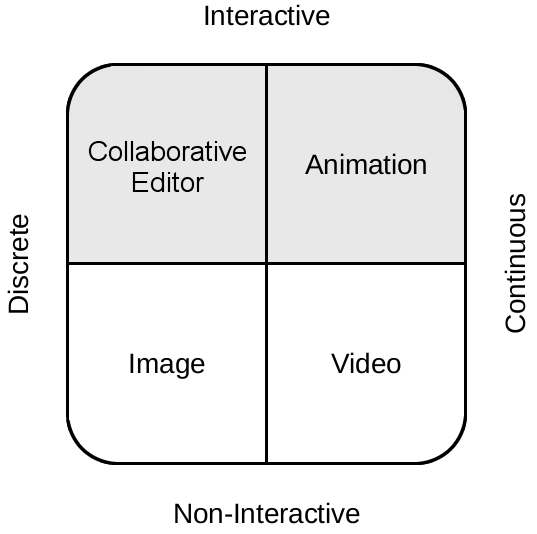
\includegraphics[width=0.4\textwidth]{figures/media_types.png}
	\caption{Media Types}
\end{figure}
	For example, an image is non-interactive and discrete, while a video is continuous and non-interactive. A simple collaborative editor with just text is interactive and discrete. An animation that changes in function of user behavior is interactive and continuous.

	Streaming protocols like \ac {RTP} and \ac{RTSP} were designed for continuous and non-interactive media types, such as audio and video. Discrete and non-interactive media don't need to be streamed through \ac{RTP} because they don't change with time. For example, if an image appears in a specific time interval, just the \ac{HTML} or \emph{JavaScript} that will reference the image must be streamed, the image itself is then transferred through \ac{HTTP}.

	In order to play a stream, a player must be prepared to interpret the stream content. For interactive stream the player must download an environment, decode the \ac{RTP} payload to determine the state and display it to the user. Streaming interactive media like a combination of \ac{HTML}, \ac{CSS} and JavaScript requires more than interpreting the code: a streamed user interface may contain an internal state that is not shown on code.
        %RP não percebi
        

 \subsection{Recording and Streaming Interactive Media}\label{intrecord}~\\
    Mauve et al. proposed an \ac{RTP} profile for real-time transmission of interactive media\cite{interactive_stream}. This new profile reuses much of video and audio profile implementation, integrating the interactive component. Hilt et al. explained how to record interactive video with this new profile \cite{interactive_record}.
        %RP não uses a citação como sujetio das frases. O trabalho não tem um nome?

	Every time an event is processed on one of the endpoints, both sender and receivers state must stay synchronized, otherwise events may behave differently.
	To achieve synchronization of interactive data, most packets have three types: \emph{State}, \emph{Delta-State} and \emph{Event}. State packet defines the environment complete state. Delta-State packets transports just the piece of state that changed. Event packets informs that an event occurred over the interactive media. 
%RP referencia?
%HR vem dos senhores de cima  (Mauve e Hilt), isto estava mal organizado

	An \ac{RTP} recorder can have two operation modes, recording or playback. Traditional \ac{RTP} players can do random access, in contrast, interactive \ac{RTP} players must restore the environment and context at a given time. The environment is the initial state, so we can call it a non-interactive discrete media and handle it over \ac{HTTP}. After the receiver has received the environment, it should calculate the state at the given time. 

	If the \ac{RTP} recorder controls the correct data to send to the receivers, it cannot be a simple \ac{RTP} recorder as it must compute the state or delta-state to send. Therefore, if the receiver receives all recorded packets, it can calculate the current state from the previous complete state. Streaming too many complete states results on more precise random accesses, but the trade-off is the higher bandwidth usage and used storage space on the recording server. On the other hand, if there are fewer complete states recorded followed by delta-states, the recorded stream will occupy less storage space, but random accesses will be less granular.
        %RP aqui já falas em recording servers, que é um conceito que ainda não apresentaste.
        %RP isto não parece um estado da arte. Não há referências e é tudo ``we''. pelo que parece ser apenas a tua opinião.
        %RP esta secção precisa de ser revista em profuncidade. Os paragrafos fazem sentido mas não há continuidade entre eles. Parece que vais saltando entre ideias e conceitos. Tens de ser melhor organizado, dividido em sub-secções que devem começar com uma explicação do problema que vai ser discutido.
	It is possible to restore the media state even if messages are lost by recording and streaming the interactive media's complete state periodically.

	In order to synchronize an interactive application state amongst participants, the needed objects to synchronize must be serializable and sent to other participants.

	Mauve et al. concluded that the ability to extract the objects state in order to synchronize them and the ability to intercept events in order to control remote objects can be realized using the \ac{MVC} concept\cite{interactive_stream}.
%RP are realized ou ``can be realized''?
        This concept separates three components within an application. The \emph{Model} represents the information itself. The \emph{View} component shows the \emph{Model} to the user in a suitable and interactive way. The \emph{Controller} represents an action from the user to the \emph {Model}. 

	Using the \ac{MVC} concept will it make possible to implement an interactive \ac{WebRTC} application that records, play, fast forward, fast rewind, stop and jump to random positions.
        %RP porquê RTP aplication? Ainda não disseste porque tem de ser RTP! Não era webrtc?
        
    

  \subsection{Collaborative Environment}\label{collabenv}~\\
	\emph{Google Wave} was a distributed collaboration platform based on \emph{Jupiter}\cite{jupiter} that adopted \ac{OT} techniques.
        	\ac{OT} technology was originally developed for consistency maintenance and concurrency control over distributed objects, \ac{OT} algorithms are mainly used in collaborative applications such as distributed document edition.
    Other Google products, such as Google Docs, are also using this type of technology. In 2010 Google stopped the development of Google Wave and released the main components as Open Source code to Apache, the project is currently known as \emph{Apache Wave} and the reference implementation is named as \emph{Wave in a Box}.
                %RP acho que o google wave merecia uma descrição mais detalhada. Mas não era aqui. Vê o comentário no final

    Among other platforms and libraries we present \emph{ShareJS}\footnote{\url{http://sharejs.org/}(accessed June 2, 2015).}, \emph{TogetherJS}\footnote{\url{http://togetherjs.com/}(accessed June 2, 2015).}, \emph{Goodow}\footnote{\url{http://realtimeplayground.goodow.com/}(accessed June 2, 2015).}, \emph{Etherpad Lite}\footnote{\url{https://github.com/ether/etherpad-lite}(Accessed 20 March 2016)} and \emph{otJS}\footnote{\url{http://operational-transformation.github.io}(accessed March 10, 2016)}.

	\emph{ShareJS} is an \ac{OT} \emph{JavaScript} library, developed by the ex \emph{Google Wave} engineer Joseph Gentle, for collaborative text and \ac{JSON} documents edition in real-time. {\color{blue} It uses \emph{ShareDB} \footnote{\url{https://github.com/share/sharedb}(accessed March 10, 2016)} for its backend and data model, which supports simple integration with any database. One of \emph{ShareDB}'s integration is over \emph{MongoDB}\footnote{\url{https://github.com/share/sharedb-mongo}(accessed March 10, 2016)}}.

	\emph{TogetherJS} is a JavaScript library that uses \ac{WebRTC} for collaborative web applications. It uses \ac{JSON} messages for \ac{OT} concurrency control but it does not provide storage. {\color{blue}\emph{TogetherJS} uses its own servers for the signaling phase and it supports microphone and mouse sharing between users. It requires a simple server (also known as hub) that echoes messages between clients, all the synchronization work is performed by the clients. Altough the hub's reduced complexity, \emph{TogetherJS}'s server is implemented with \emph{NodeJS}, if we would not choose \emph{NodeJS} for server implementation we would need read the hub's source code and understand what changes are needed to perform on our web server in order to make it compatible with \emph{TogetherJS}.}

	\emph{Goodow} is a collaborative framework with its own server implementation, it supports four types of collaborative elements: String, Lists, Maps and Custom objects.
        %RP estes 3 últimos parágrafos estão desligados do resto. O que pretendes apresentar?
	

	{\color{blue}\emph{Etherpad Lite} is a collaborative text editor implemented with \emph{NodeJS} that allows not only the text operations but also to associate authorships to pieces of text. It supports adding functionality trought plugins\footnote{\url{http://static.etherpad.org/plugins.html}(Accessed 20 March 2016)}, for example:
		\begin{itemize}
		\item exporting and importing document formats such as \emph{DOC}, \emph{PDF}, \emph{ODT} and \emph{DOCX}.
		\item painting and drawing.
		\item video and audio chat using WebRTC.
		\item create slideshows.
		\item spell checking.
		\item text to speech.
		\end{itemize}
	}



	{\color{blue}\emph{otJS} is a \emph{JavaScript} library that only implements operation transformations on client side over plain text. An implication of implementing just the client side is the extra effort that is necessary to implement content's persistent storage, besides this drawback this library is very flexible because it's not tied to a specific database or server side technology.}
	


\begin{table}[H]
\centering

\label{my-label}
\begin{tabular}{|c|c|c|c|}
\hline
\textbf{Library} & \textbf{Own Server} & \textbf{Own Storage} & \textbf{Operations} \\ \hline
ShareJS          & yes                 & yes                  & text+objects        \\ \hline
TogetherJS       & yes                 & no                   & text+objects        \\ \hline
Goodow           & yes                 & yes                  & text+objects        \\ \hline
Etherpad Lite    & yes                 & yes                  & extendable 			    \\ \hline
OT.js            & no                  & no                   & text                \\ \hline
\end{tabular}
\caption{Comparision between Operational Transformation libraries}
\end{table}


        %RP falta falar um pouco das ferramentas de colaboração já existentes? Wave, Hangouts, skype, etc? Acho que isto merecia uma secção à parte, mesmo que mais curta.
